

\subsubsection{Amministratore: Vista dei Casi d'Uso}
Riportiamo qui di seguito le funzioni che andremo a contestualizzare all'interno
del Dominio del nostro problema, e descritti nella SottoSottosezione \vref{subsubsec:adminucaseview}:
\begin{itemize}
\diam \texttt{getFreeSlotsAfter}
\diam \texttt{fetchReservations}
\diam \texttt{addReport}
\diam \texttt{postponeReservs}
\diam \texttt{Reserve}
\diam \texttt{fetchPendantReq}
\diam \texttt{Login}
\diam \texttt{fetchRemoveReq}
\diam \texttt{fetchPostponeReq}
\diam \texttt{destroyRequestPostpone}
\diam \texttt{freeSlotReserv}
\end{itemize}



\begin{figure}[p]
 \centering
   \subfloat[][\emph{1. getFreeSlotsAfter}.]{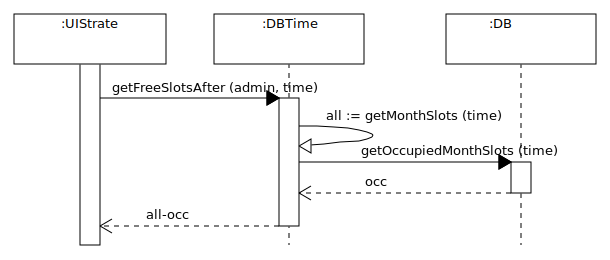
\includegraphics[scale=0.6]{svgs2/01getFreeSlots}}\\
   \subfloat[][\emph{2. fetchReservation}.]{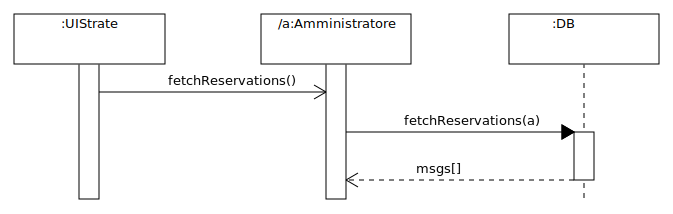
\includegraphics[scale=0.6]{svgs2/02fetchReservation}}\\
   \subfloat[][\emph{6. fetchPendantReq}.]{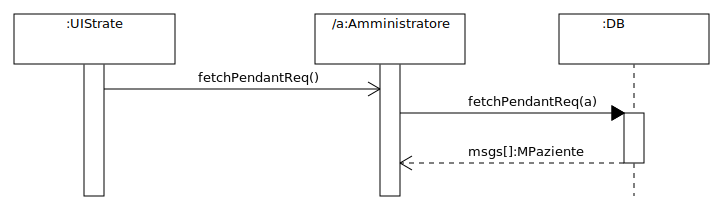
\includegraphics[scale=0.6]{svgs2/06fetchPendantReq}}\\
   \subfloat[][\emph{8. fetchRemoveReq}.]{\includegraphics[scale=0.5]{svgs2/08fetchRemoveReq}}\\
   \subfloat[][\emph{9. fetchPostponeReq}.]{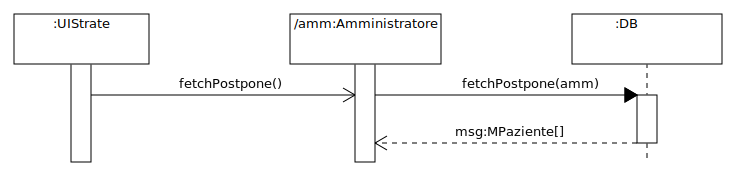
\includegraphics[scale=0.5]{svgs2/09fetchPostponeReq}}\\
 \caption{\emph{Use Case Realization for Admin's view (1)}}
\end{figure}

\begin{description}

\item[getFreeSlotsAfter]

Possiamo evidenziare come questa operazione richieda un accesso al database,
per ottenere quali siano gli slots occupati. Tuttavia dobbiamo sottolineare
come, all'interno della base di dati che memorizzerà permanentemente le
operazioni, siano memorizzati per ovvie ragioni solamente i dati relativi agli
slot occupati, e non quelli liberi. Conseguentemente, è necessario effettuare
un computo ulteriore dopo aver prelevato gli slots occupati lato database:
la responsabilità di questo computo tuttavia non può essere delegato ad
\texttt{DBAdmin}, per non attribuire anche il compito di effettuare la gestione
del tempo. In questo caso si rende quindi necessario aggiungere una classe 
accessoria \texttt{DBTime}, che medi con la precedente per effettuare un primo
computo degli \texttt{Slot} temporali liberi.
\bigskip

\item[fetchReservation]

In questo caso facciamo utilizzo del GRASP \textbf{Expert}, in quanto ci chiediamo
quale sia l'elemento che contenga le informazioni relative a quale sia l'amministratore
corrente nel sistema. Questa risposta ci viene fornita dalla classe 
\texttt{Amministratore}. Inoltre, allo scopo di effettuare il \textbf{Principio di
Separazione Controllo-Interrogazione}, identifichiamo una funzione
$fetchReservations(:admin)$ verso la \texttt{DBAdmin}, la quale si occupa di ottenere
il risultato senza modificare lo stato di \texttt{Amministratore} (interrogazione), 
ed attribuiamo alla funzione in discussione un comando, che invece ne effettua 
la modifica di stato. 

In questo caso, la classe \textbf{Expert}, identifica in qualche modo anche l'oggetto
radice del nostro sistema. Considerazioni analoghe possono essere effettuate
per i contratti \texttt{fetchPendantReq} (\textbf{Contratto 06}), \texttt{fetchPostponeReq}
(\textbf{Contratto 08}) e \texttt{fetchPostponeRew} (\textbf{Contratto 09}), che conseguentemente
non tratteremo, visto che il problema che si presenta in questi contesti è
risolvibile in un modo del tutto identico con quello già enunciato.
\bigskip

\item[addReport]

In questo caso, obbiediendo al GRASP \textbf{Controller}, l'oggetto che è ricevitore
del comando di questo contratto è la stessa \texttt{Prenotazione}: possiamo quindi
trasformare la funzione $addReport(\alpha,\beta)$ nel metodo $\alpha.addReport(\beta)$:
questa operazione modificherà lo stato interno dell'oggetto, che verrà aggiornato
a sua volta all'interno del database.
\bigskip

\begin{figure}[!thp]
 \centering
   \subfloat[][\emph{3. addReport}.]{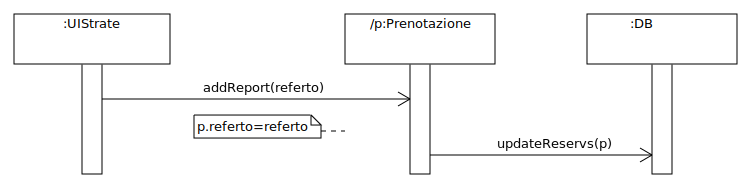
\includegraphics[scale=0.6]{svgs2/03addReport}}\\
   \subfloat[][\emph{4. postponeReservs}.]{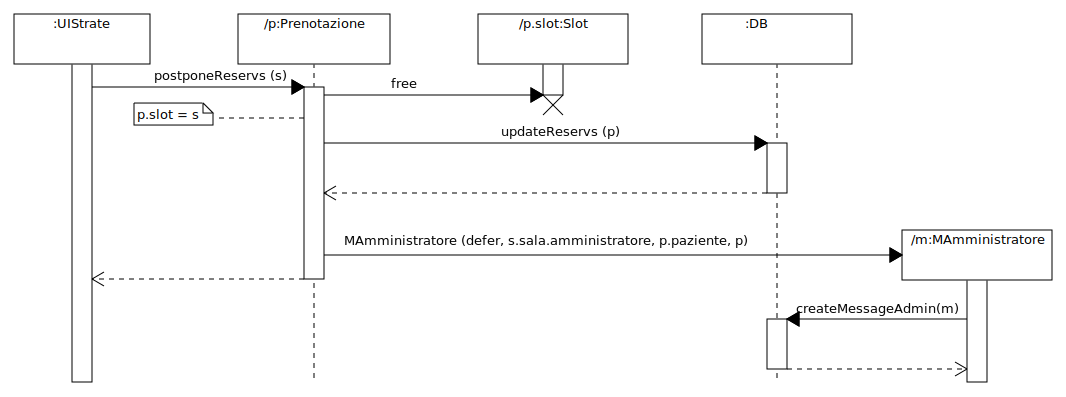
\includegraphics[scale=0.5]{svgs2/04postponeReservs}}\\
   \subfloat[][\emph{5. Reserve}.]{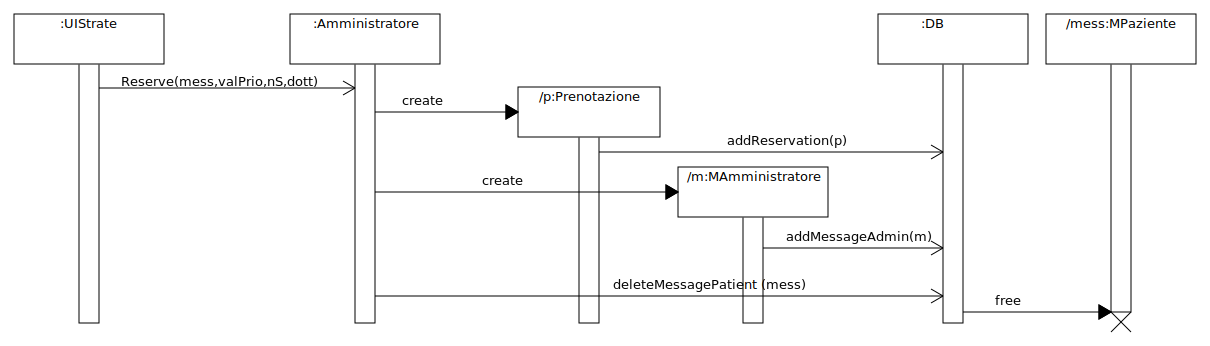
\includegraphics[scale=0.5]{svgs2/05Reserve}}\\
   \subfloat[][\emph{10. destroyRequestPostpone}.]{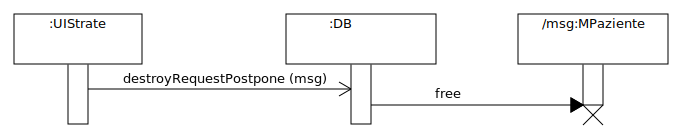
\includegraphics[scale=0.5]{svgs2/10destroyRequestPostpone}}\\
   \subfloat[][\emph{11. freeSlotReserv}.]{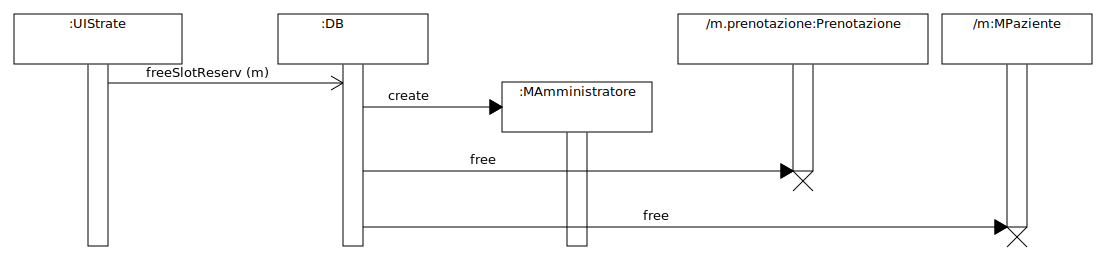
\includegraphics[scale=0.5]{svgs2/11freeSlotReserv}}\\
 \caption{\emph{Use Case Realization for Admin's view (2)}}
\end{figure}

\item[postponeReservs]

In ottemperanza all'osservazione effettuata precedente, trasformiamo la 
funzione $postponeReservs(\alpha,\beta)$ in modo analogo nel metodo $\alpha.postponeReservs(\beta)$.
In particolare possiamo osservare tramite il diagramma associato come si possano
creare oggetti all'interno del database (ovvero creando prima l'oggetto, e 
trasferendolo successivamente ad una funzione gestita dal framework), e come
sia possibile eliminarli (ovvero tramite il passaggio di un'istanza dell'oggetto
stesso che si conosce essere contenuto come record di una tabella del database).
\bigskip

\item[Reserve]

In questo caso abbiamo che l'elemento radice del nostro sistema è effettivamente
la classe \texttt{Amministratore}: in questo modo è inoltre possibile semplificare
la procedura di estrazione dell'amministratore (informazione contenuta all'interno
della classe stessa), senza doverla per forza ottenere dal messaggio in lettura.
\bigskip



\item[destroyRequestPostpone]

In questo caso abbiamo che l'oggetto che rappresenta il sottosistema principale,
sempre in obbedienza al principio \textbf{Controller}, è di fatti la stessa classe
\texttt{DBAdmin}: l'unico compito che vi si richiede è di fatti quello dell'eliminazione
del messaggio.
\bigskip

\item[freeSlotReserv]

Analogamente a quanto discusso precedentemente, la classe bf{Controller} è ancora
\texttt{DBAdmin}: in questo caso tuttavia si aggiunge una responsabilità alla
classe, che è quella della creazione del messaggio, che comunque richiede
l'interazione con il framework EJP.

\begin{figure}[!thp]
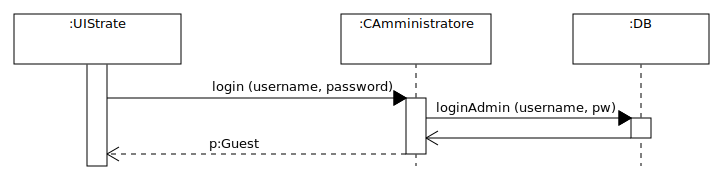
\includegraphics[scale=0.4]{svgs2/07Login}
\caption{\textit{Login - Use Case Realization for Admin's view (3)}}
\end{figure}

\item[Login]

Analogamente a quanto discusso precedentemente, la responsabilità nell'effettuazione
della procedura di Login è affidata alla classe costruttruce (\textbf{Creator}) CAmministratore,
in quanto ha la responsabilità di ottenere le istanze di Amministratori.
 
\end{description}

Possiamo a questo punto mostrare in Figura \vref{fig:firstdmrevision} una seconda
versione del Modello di Business: per praticità di lettura abbiamo preferito
tenere in questa versione unicamente i metodi propri di ogni singola classe,
diversamente da quanto già effettuato in Figura \vref{fig:firstdmrevision}.

\begin{figure}[p]
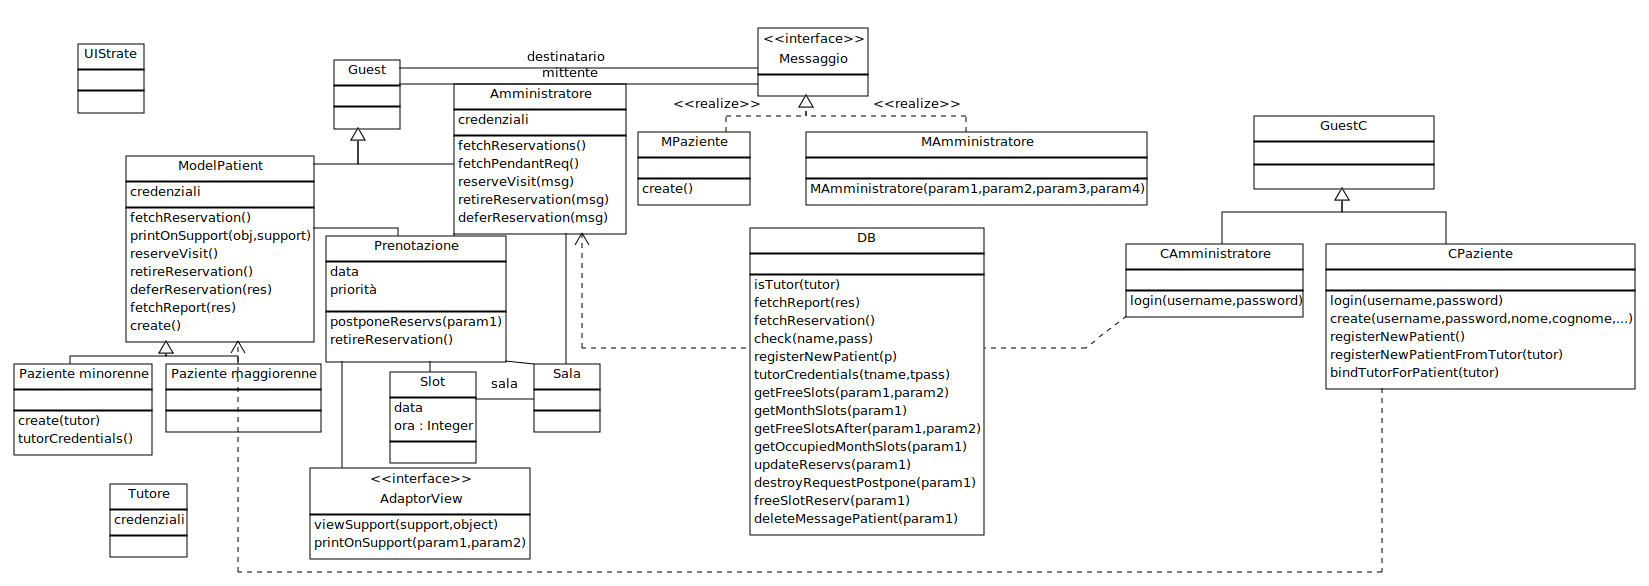
\includegraphics[scale=0.5,angle=90]{svgs2/modellodiDominio}
\caption{\textit{Second Revision of the Domain Model presented in Section \vref{sec:domainmodel}}, with only methods.}
\label{fig:firstdmrevision}
\end{figure} 

